\documentclass{article}
\setlength{\oddsidemargin}{0in}
\setlength{\evensidemargin}{0in}
\setlength{\textwidth}{6.5in}
\setlength{\parindent}{0in}
\setlength{\parskip}{\baselineskip}

\usepackage{amsmath,amsfonts,amssymb,geometry}
\usepackage{graphicx}
\usepackage{fancyhdr}
\usepackage{ulem}
\usepackage{listings}
\pagestyle{fancy}
\setlength{\headheight}{15pt}

\begin{document}

CSCI 3104-300 Summer 2019 \hfill Problem Set 5 \\
Hoffman, Ryan \\
01/11

\hrulefill

\vspace{-3mm}
\begin{enumerate}
    
	\item (60 points) 
	\begin{enumerate}

	\item From scratch, implement the functions \par
	{\tt alignStrings}, {\tt extractAlignment}, and {\tt commonSubstrings}. 
	You may not use any library functions that make their implementation trivial. 
	Within your implementation of {\tt extractAlignment}, ties must be broken uniformly at random.
	
	Submit (i) a paragraph for each function that explains how you implemented it (describe how it works and how it uses its data structures), and (ii) your code implementation, with code comments. \label{q:align:code}
	
	Hint: test your code by reproducing the {\tt APE} / {\tt STEP} and the {\tt EXPONENTIAL} / {\tt POLYNOMIAL} examples in the lecture notes (to do this exactly, you'll need to use unit costs instead of the ones given above).
	\textbf{Solution:}\par
	{\tt alignStrings(x,y)}, as explained in the pseudo code, takes as input two ASCII strings $x$ and $y$, and runs a 
	dynamic programming algorithm to return the cost matrix $S$, which contains the optimal costs for all the subproblems 
	for aligning these two strings. It was implemented by following the pseudo code given. Here is my code:\par
	\begin{lstlisting}
	def alignStrings(x,y):
		nx = len(x)
		ny = len(y)
		# Initialize S, table of length nx by ny
		S = [0]*(ny+1)
		for i in range(ny+1):
			S[i] = [0]*(nx+1)
		# Base cases: first column and first row
		for i in range(nx+1):
			S[0][i] = i
		for j in range(ny+1):
			S[j][0] = j
		# Optimal cost for x[0..i] and y[0..j]
		for j in range(1,nx+1):
			for i in range(1,ny+1):
				S[i][j] = cost(S,x,y,i,j)
		return S
	\end{lstlisting}
	\par
	\textbf{Solution:}\par
	{\tt extractAlignment(S,x,y)} takes as input an optimal cost matrix $S$, strings $x,y$, and returns a vector $a$ that represents an optimal sequence of edit operations to convert $x$ into $y$. 
	This optimal sequence is recovered by finding a path on the implicit DAG of decisions made by {\tt alignStrings} to obtain the 
	value $S[n_{x},n_{y}]$, starting from $S[0,0]$. This function was implemented using the given pseudo code. Here is my code:\par
	\begin{lstlisting}
	# S is an optimal cost matrix from alignStrings
	def extractAlignment(S,x,y):
		#Initialize a, an empty list of edit operations
		a = []
		# Initialize the search for a path to S[0,0]
		[i,j] = [len(y),len(x)]
	
		while (i > 0 or j > 0):
			# what was an optimal choice?
			a.append(determineOptimalOp(S,i,j,x,y))
			# move to next position
			[i,j] = updateIndices(S,i,j,a)
		return a
	\end{lstlisting}\par
	I wasn't able to figure out a solution to the code for {\tt commonSubstrings}.\par

	\item Using asymptotic analysis, determine the running time of the call \par 
	{\tt commonSubstring(x,L,extractAlignmnt(alignString(x,y),x,y))}\par
	Justify your answer.\par
	\textbf{Solution:}\par
	I think the asmptotic runtime for the above function call would be $\Omega(n)$. Because it takes the inputs and finds the common substrings. 
	\item String alignment algorithms can be used to detect changes between different versions of the same document (as in version control systems) or to detect verbatim copying between different documents (as in plagiarism detection systems).
	
	The two {\tt data\_string} files for PS5 (see class Moodle) contain actual documents recently released by two independent organizations. Use your functions from~\eqref{q:align:code} to align the text of these two documents. 
	Present the results of your analysis, including a reporting of 10 of the longest substrings in $x$ of length $L=20$ or more that could have been taken from $y$, and briefly comment on 
	whether these documents could be reasonably considered original works, under CU's academic honesty policy.\par
	\textbf{Solution:}\par
	I wasn't able to properly implement the functions in part (a). However, I believe that 
	the works could be considered original works under CU's academic honesty policy because they do require a percentage threshold 
	to be in this category. This means that ANY paper or work could be challenged for it's originality by the owner and it is a process 
	that is open to interpretation.\par
	\end{enumerate}
	
	\pagebreak
    
	\item (10 points) Shadow is trying to figure out all the potential paths from the bank he is trying to rob to the party's hideout, given by the network below.  Help him calculate the number of paths from node 1 to node 14.
	
	Hint:\ assume a ``path'' must have at least one edge in it to be well defined, and use dynamic programming to fill in a table that counts number of paths from each node $j$ to 14, starting from 14 down to 1.

    \begin{figure}[h!]
        \centering
        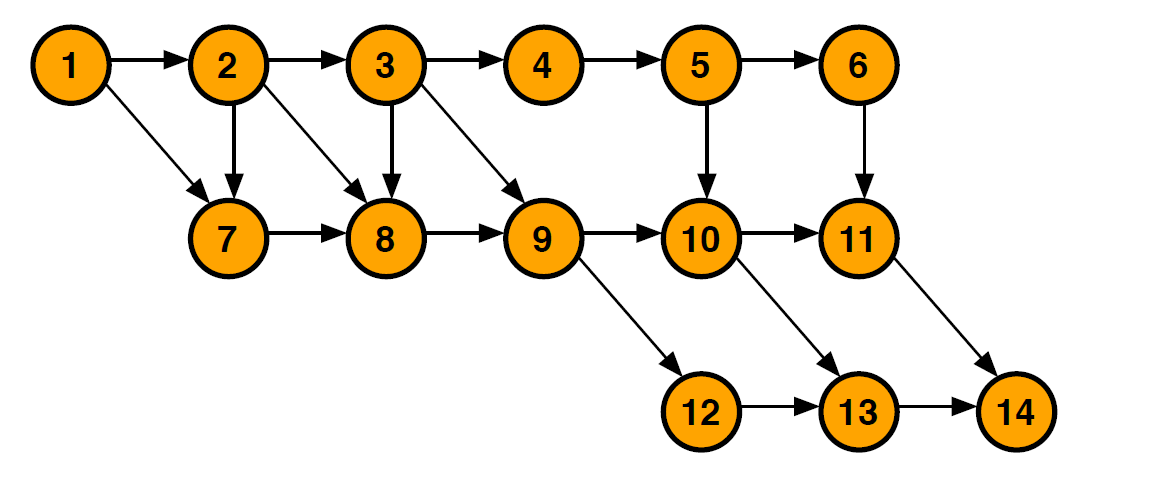
\includegraphics[scale=0.4]{graph.png}
        \caption{Thormund's Network}
        \label{fig:my_label}
    \end{figure}
	\textbf{Solution:}\par
		I counted the number of paths to be 18. I don't know how to use the hint, so I just counted the paths by hand.
    \pagebreak
    
	\item (20 points) As a new event in the Triwizard Tournament, students must compete in pairs in the following game. An even number $n$ of magical items are laid out in a row, with the $i$-th item having a value of $v(i)$ in Knuts for each $i=1,2,\dotsc,n$. The players alternate turns, and on each turn, the player may choose either the first item or the last item remaining in the row, then remove it from the row and add it to their pile. The player with the highest-valued pile at the end wins. (The value of a player's pile at the end is simply the sum of the value of the items in the pile.) We will use dynamic programming to help us analyze this game.
	
	\begin{enumerate}
	\item For a given vector $v$ of values, let $F(i,j)$ denote the maximum value that the first player can definitely achieve using the values $v[i], \dotsc, v[j]$---this means a \emph{tight}, \emph{exact} upper bound, an amount which the first player cannot beat, but that the first player can in fact achieve if he/she plays optimally. Write down a recurrence relation for $F(i,j)$ and prove that it is correct. Be sure to include a base case!  You can assume that this problem has optimal substructure.\par
	\textbf{Solution:}\par
	I really wish I knew how to answer this question but I have no idea how to write a recurrence relation for F(i,j) and prove that it's correct.\par
	\item Based on your recurrence from part (a), describe a dynamic programming table and the order in which it should be filled in.\par
	\textbf{Solution:}\par
	I wasn't able to do part (a) and therefore I have no solution to this part. \par	
	\item Write pseudo-code for the dynamic programming solution you described in part (b) and analyze its run-time.\par
	\textbf{Solution:}\par
	Also, not able to solve this part. 
	\end{enumerate}

\end{enumerate}
\end{document}